\chapter{Task 6}
\label{chapter:task6}
An N dimensional equispaced array antenna  with identical elements was considered in this section. Having an equispaced array antenna simplifies the computations as we know that the phase difference between the elements will be the same for every element (i.e. constant phase difference).

The positions, $\{\mathbf{r}_n\}_{i=1}^N$, of the antennas can be written as  
\begin{equation}
\mathbf{r}_n = \mathbf{r}_c + a_n \hat{a} = \mathbf{r}_c + \left (n + \frac{N+1}{2}\right)d\hat{a}
\end{equation}
where $\mathbf{r}_c$ is the center of the array and we have intermediate  spacing d the total length is then Nd and we may write the electrical field as 
\begin{equation}
\mathbf{E}_n(\mathbf{r}) = \frac{e^{-jkr}}{r} \mathbf{G}(\mathbf{r}).
\end{equation}
We have earlier defined the far field function and the array  factor in section \ref{chapter:task4}, which now allows us to consider the array factors and the radiation patterns. If the antenna is directed at an angle $\theta$  the array factor can be written as 
\begin{align}
&AF = 1 + e^{j(kd\cdot 1 cos(\theta) +\alpha)}  + ... + e^{j\cdot(N-1)(kdcos(\theta) +\alpha)} = \\ & \sum_{n=1}^N  e^{j(kd\cdot (n-1)) cos(\theta) +\alpha)} = e^{j(N-1)\Psi/2}sin(N\Psi/2)/ sin(\Psi/2)
\end{align}
where $\Psi = \alpha + kdcos(\theta)$ and assuming that the elements of the antenna are equal.

\section{Task 6 a}
In this section the array antenna with 5 elements was considered for intermediate element spacing $d = \lambda/4$ pointed in the H-plane. Firstly the theory regarding the array antennas and the H-plane will be presented. Then the results from the MATLAB simulations will be presented. 
\subsection{Theory}
The total radiation pattern of an array antenna is defined as  
\begin{equation}
Pattern_{radiation}^{tot} = (\text{element radiation pattern})\times(AF).
\end{equation}
 For an equispaced array with intermediate spacing d and N-1 elements there will be a phase difference $\alpha$ between every element. The normalized array factor can the be written as 
\begin{equation}
|AF| = sin(N\Psi/2)/( N sin(\Psi/2) ).
\end{equation}
where $\Psi = \alpha + kdcos\theta$.  As we are considering horizontal dipole antennas the radiation pattern in the far field region will be 
\begin{equation}
f = \sqrt{1-sin^2(\theta)cos^2(\phi)}
\end{equation}
A maximum of the array factor can be found at $\Psi$ =0 which corresponds to $\alpha = kdcos(\theta_0)$ where $\theta_0$ is called the steering angle. This will simplify the expression when the array antenna is directed at a specific region. The radiation patterns the total radiation pattern can thus be plotted in the H plane  which corresponds with $\alpha = kdcos(\theta_0) =kd$, i.e. $\theta_0 =0$\cite{AntennasFundamentals}. \cite{kildal2000foundations}

The radiation pattern, far field pattern may be normalized and plotted in dBi as described in chapter \ref{chapter:task3}.

\subsection{Results}
The MATLAB scripts for the simulation if the H-plane can be viewed in appendix \ref{section:task6a.m}. The plotted results for  the radiation-, far field- and AF-patterns were plotted in figures \ref{task6a:ypol}, \ref{task6a:ypolHpat} and \ref{task6a:ypolAF}, respectively. 

\begin{figure}[h]
\centering
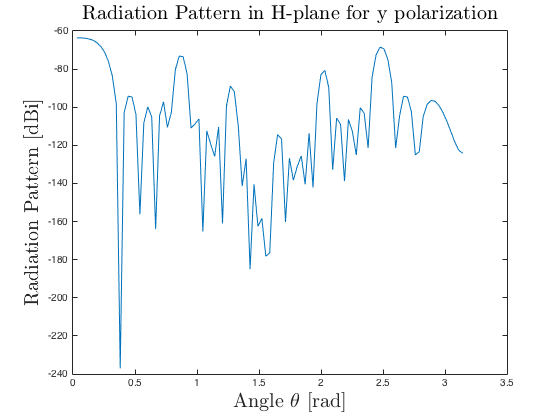
\includegraphics[scale=0.4]{/Users/marikasvensson/Documents/MATLAB/MicroProject/finished/task6/6a/ypolHplane.png}
\caption{This figure shows the radiation pattern as a function of $\theta$in the H-plane}
\label{task6a:ypol}
\end{figure}

\begin{figure}[h]
\centering
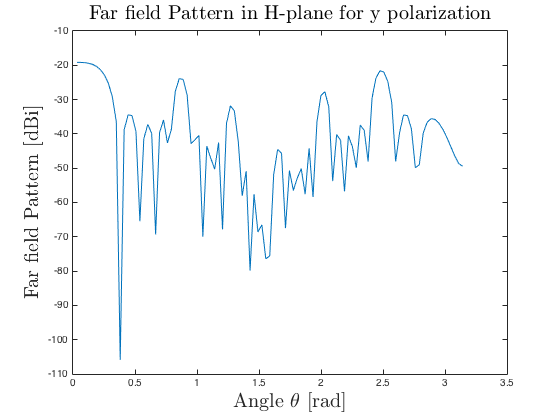
\includegraphics[scale=0.4]{/Users/marikasvensson/Documents/MATLAB/MicroProject/finished/task6/6a/ypolHplanePattern.png}
\caption{This figure shows the far field pattern as a function of $\theta$in the H-plane}
\label{task6a:ypolHpat}
\end{figure}

\begin{figure}[h]
\centering
\includegraphics[scale=0.4]{/Users/marikasvensson/Documents/MATLAB/MicroProject/finished/task6/6a/ypolAF.png}
\caption{This figure shows $AF$ as a function of $\theta$ and $\phi$ for y polarized dipoles}
\label{task6a:ypolAF}
\end{figure}
\FloatBarrier

\section{Task 6 b}
In this section the array antenna with 5 elements was considered for intermediate element spacing $d \in \lambda[1/4,4]$ pointed in the broadside direction. Firstly the theory regarding the array antennas and the broadside will be presented. Then the results from the MATLAB simulations will be presented. 
\subsection{Theory}
Consider the theory in task 6a, this is  the theory which is needed to compute the  result here as well but with some small adjustments. 
The radiation patterns the total radiation pattern can be plotted in the broadside, this corresponds with $\alpha = kdcos(\theta_0) = 0 $. The steering angle is thus $\theta_0 = \pi/2$. \cite{kildal2000foundations}

\subsection{Results}
The MATLAB scripts for the simulation if the H-plane can be viewed in appendix \ref{section:task6a.m}. The plotted results for  the radiation- , far field- and AF-patterns were plotted in figures \ref{task6b:ypol}, \ref{task6b:ypolHpat} and \ref{task6b:ypolAF}, respectively. The figures illustrates the radiation pattern for d $\in \lambda[1/4, 4].$ 

\begin{figure}[h]
\centering
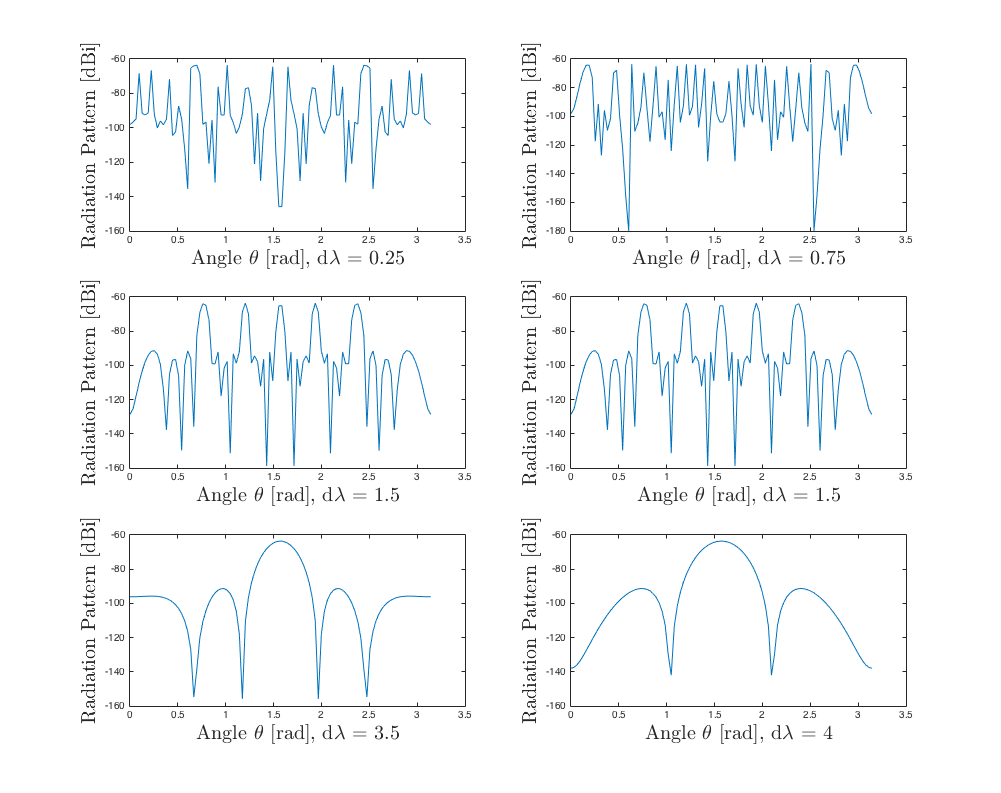
\includegraphics[scale=0.5]{/Users/marikasvensson/Documents/MATLAB/MicroProject/finished/task6/6b/ypolbroad.png}
\caption{This figure shows the radiation pattern as a function of $\theta$ for y polarized dipoles in an array}
\label{task6b:ypol}
\end{figure}

\begin{figure}[h]
\centering
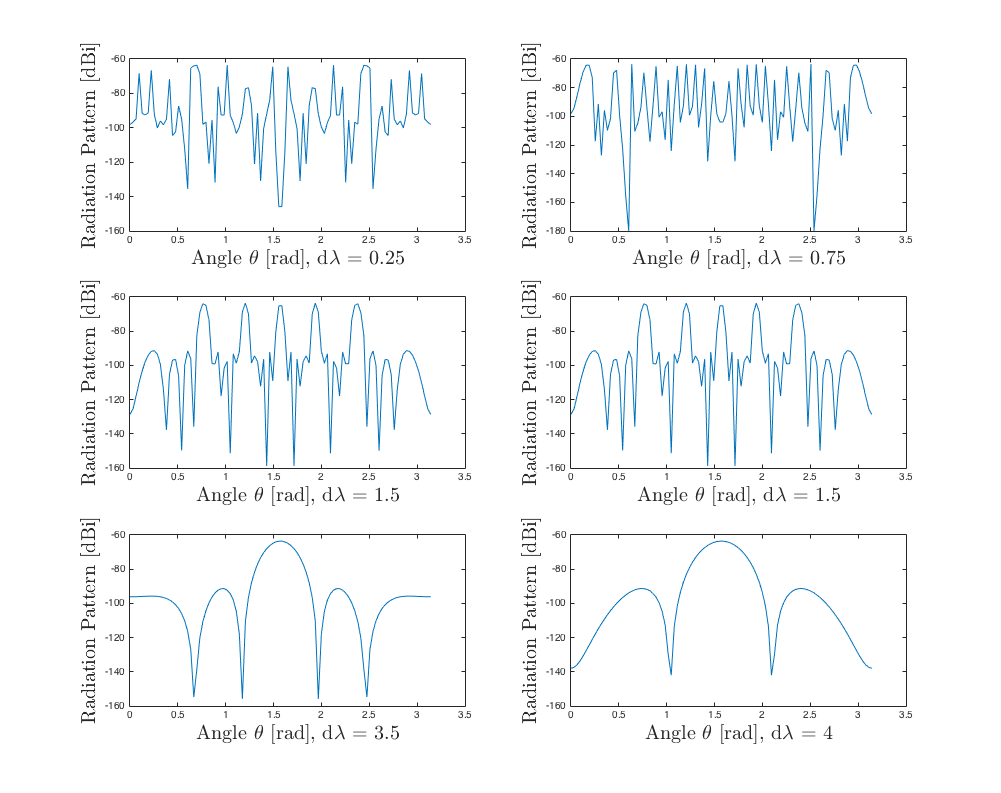
\includegraphics[scale=0.5]{/Users/marikasvensson/Documents/MATLAB/MicroProject/finished/task6/6b/ypolbroad.png}
\caption{This figure shows the far field pattern as a function of $\theta$ for y polarized dipoles in arrays}
\label{task6b:ypolHpat}
\end{figure}

\begin{figure}[h]
\centering
\includegraphics[scale=0.5]{/Users/marikasvensson/Documents/MATLAB/MicroProject/finished/task6/6b/ypolAF.png}
\caption{This figure shows $AF$ as a function of $\theta$ and $\phi$ for y polarized dipoles}
\label{task6b:ypolAF}
\end{figure}


